\section{The state as a shortcut}
\label{sec:shortcut}
\label{sec:confound}

Many tactile datasets record each object in a separate session, and in our training data each material appears under only one hardware configuration, a sensor unit and its gel. The hardware signature in an image then points to a subset of the classes, and a classifier can use it to narrow its predictions without relying on texture alone.

\paragraph{On our recordings.}
In June and July, unit 2 recorded only four of the 20 materials. All September and October recordings were collected with unit 2, including materials previously recorded with unit 1. A ResNet-50 trained on June and July assigns \XpIntroUnitTwoShare\pct\ of these test episodes to the four classes associated with unit 2. Its accuracy on the sixteen materials recorded with unit 1 in training is only \XpIntroUnitAcc\pct, compared with 5\pct\ chance accuracy. Frozen Sparsh encoders~\cite{higuera2024sparsh} show the same failure (\supp{H}), and the state is easy to read from pretrained features. A linear probe tells our two units apart from a single crop of held-out materials at \ProbeIjepaRawUnit\ to \ProbeSdinoRawUnit\pct\ for the three Sparsh encoders and \ProbeDinovRawUnit\pct\ for DINOv2 (\supp{R}).

\paragraph{Adding the new unit to the training set.}
Changing the training set confirms the cause. On the 13 materials common to every split, a CNN trained on campaign A scores \ThirteenAtoBRaw\pct\ on campaign B, recorded on the same hardware, and \ThirteenAtoDRaw\pct\ on campaign D, recorded on the other unit. Training on A and B gives \ThirteenABtoDRaw\pct\ on D. Adding campaign C, which brings the new unit into the training set with only four materials, lowers this to \ThirteenABCtoDRaw\pct. With the state removed (\cref{sec:method}), the same model scores \ThirteenABCtoDPrev\pct\ (\supp{Q}).

\begin{figure}[t]
  \centering
  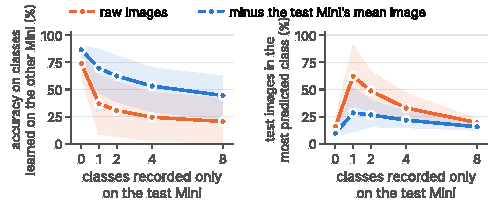
\includegraphics[width=\linewidth]{fig/fig_confound.pdf}
  \caption{\textbf{Controlled class--hardware association.} On SITR's four GelSight Minis~\cite{sitr2025} we train on $20-k$ classes recorded on one Mini and $k$ recorded only on the test Mini, and test all classes on the test Mini (frozen DINOv2, MLP head; mean over 12 Mini pairs and class draws, band: 10th--90th percentile). Orange: raw images. Blue: the test Mini's mean image subtracted (\cref{sec:second}).}
  \label{fig:confound}
\end{figure}

\paragraph{Controlled experiments on public data.}
To test whether the hardware signature drives this bias, we use SITR~\cite{sitr2025}, which records the same 20 objects with four GelSight Minis, and train with $k$ objects recorded only on the test Mini and the others only on another Mini (\cref{fig:confound}). With one such object, the classifier assigns \CfSitrRawOneTop\pct\ of the test images to it, and accuracy on the others falls from \CfSitrRawZeroCross\ to \CfSitrRawOneCross\pct. On Real Tactile MNIST~\cite{tactilemnist2025}, tying one digit to the test gel assigns \CfTmdRawOneTop\pct\ of the test contacts to that digit.

\paragraph{Implication for evaluation.}
A train/test split of the same recordings carries each hardware signature on both sides, so it rewards the shortcut and cannot reveal it. To expose the dependence, a dataset should record which unit and gel produced every image, and an evaluation should hold out hardware and report how predictions spread over classes.
